\documentclass{standalone}
\usepackage[utf8]{inputenc}
\usepackage{amsmath}
\usepackage{tikz}
\usepackage{pgfplots}
\pgfplotsset{compat=1.11}
\usetikzlibrary{shapes,snakes,shadows,arrows,calc,decorations.markings,patterns,fit,matrix,spy}
\pagestyle{empty}
\begin{document}
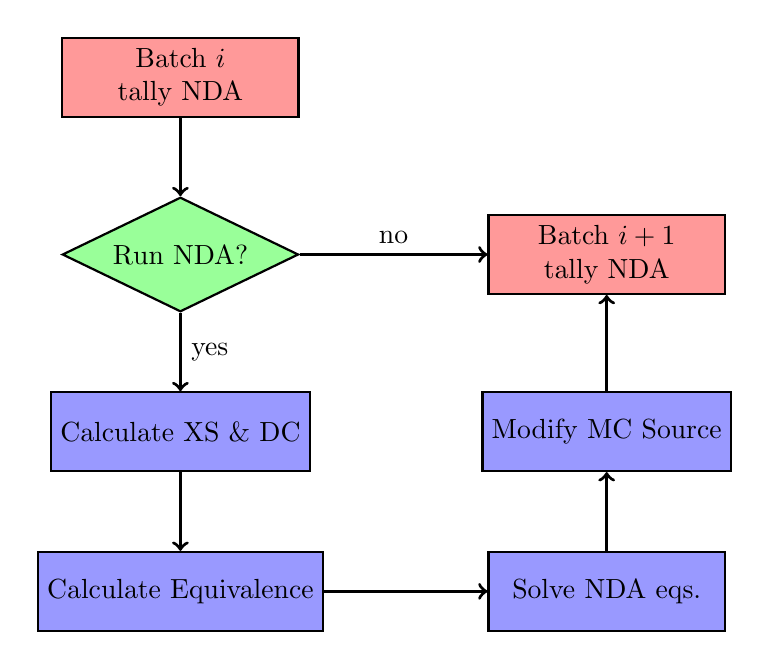
\begin{tikzpicture}
	\matrix[every node/.style={draw, thick, minimum width=3cm, minimum height=1cm, align=center}, column sep=2cm, row sep=1cm] (m) {
\node[draw, fill=red!40] (start) {Batch $i$ \\ tally NDA}; & \\
 \node[draw, diamond, aspect=2, fill=green!40] (cmfd) {Run NDA?}; & \node[draw, fill=red!40] (end) {Batch $i + 1$ \\ tally NDA};  \\
\node[draw, fill=blue!40] (xs) {Calculate XS \& DC}; & \node[draw, fill=blue!40] (modify) {Modify MC Source}; \\
\node[draw, fill=blue!40] (nonlinear) {Calculate Equivalence}; &  \node[draw, fill=blue!40] (eqs) {Solve NDA eqs.};\\
};

\begin{scope}[every path/.style={->,very thick,draw}]
        \draw (start.south) -- (cmfd.north);
        \draw (cmfd.east)  -- node[above] {no} (end.west);
        \draw (cmfd.south)  -- node[right] {yes} (xs.north);
		\draw (xs.south)  --  (nonlinear.north);
		\draw (nonlinear.east)  --  (eqs.west);
		\draw (eqs.north)  --  (modify.south);
		\draw (modify.north)  --  (end.south);
    \end{scope}

\end{tikzpicture}
\end{document}
